% !TEX root = ../main.tex
\section{Optional Rules} \label{sec::optionalrules}
\subsection*{Equipment Properties} \label{ssec::equipmentproperties1}
    Apart from their weight class, armors have specific properties.
    These carry with them beneficial and detrimental effects.
    Additionally, some feats have effects that apply to armor with certain properties, or are restricted by them.

    As usual, weapons also have properties.
    A small amount of new properties are added to the ones in the PHB.

    A list of the different armor properties is included in the equipment chapter (see page \pageref{ssec::armorproperties}).

% !TEX root = ../main.tex
\subsection*{Brutal Criticals} \label{ssec::brutalcriticals}

Presented here are optional rules that expand the scope of critical hits.
Introducing a series of critical hit charts that vary based on the damage type of the attack, this module adds an additional element of uncertainty, suspense, and surprise to combat.

\subsubsection{Revisions to Critical Hits}
    \begin{itemize}
        \item When you land a critical hit on a creature, roll the damage dice twice and add them together as normal.
        Then, roll a d20 and use the corresponding result on the critical hit chart determined by the damage type of your attack.
        \item When you score a critical hit with an attack that does two or more types of damage, choose one of those damage types and roll on that critical chart.
        \item Traits and feats like Savage Attacks and Brutal Critical continue to work as written.
    \end{itemize}

\begin{figure}[t]
    \centering
    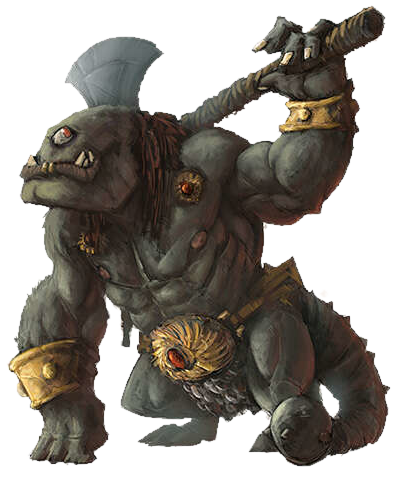
\includegraphics[width=0.47\textwidth]{03mechanics/img/41cyclops.png}
\end{figure}

\subsubsection{Damage Charts}
    \begin{DndTable}[width=\linewidth, header=Bludgeoning]{cX}
        \textbf{d20} & \textbf{Effect} \\
        1     & Roll damage as normal. \\
        2-3   & The next attack against the creature has advantage. \\
        4-6   & Push the creature up to 1 meter in any direction. \\
        7-8   & Push the creature up to 3 meters in any direction. \\
        9-11  & Attacks against the creature are made with advantage until the start of your next turn. \\
        12-13 & The creature is knocked prone. \\
        14-16 & Push the creature up to 3 meters away, and the creature is knocked prone. \\
        17-18 & Roll on the Minor Injury chart.
        If the creature is wearing heavy armor roll on the Major Injury chart instead. \\
        19    & Deal the twice maximum result of your damage dice and roll on the major injury chart. \\
        20    & Deal the maximum result of your damage dice twice, the creature is stunned until the end of your next turn, and roll on the major injury chart.
    \end{DndTable}

    \pagebreak

    \begin{DndTable}[width=\linewidth, header=Piercing]{cX}
        \textbf{d20} & \textbf{Effect} \\
        1     & Roll damage as normal. \\
        2-3   & The creature may only move half its movement speed on its next turn. \\
        4-6   & Roll damage dice twice and use the higher result. \\
        7-8   & The creature's movement speed is zero until the end of its next turn. \\
        9-11  & You can roll one of the weapon's damage dice one additional time and add it to the extra damage of the critical hit. \\
        12-13 & Roll on the minor injury chart with disadvantage. \\
        14-16 & Roll on the minor injury chart. \\
        17-18 & Roll on the major injury chart. \\
        19    & Roll on the major injury chart. \\
        20    & Roll on the minor injury chart, and roll on the major injury chart.
    \end{DndTable}

    \begin{DndTable}[width=\linewidth, header=Slashing]{cX}
        \textbf{d20} & \textbf{Effect} \\
        1     & Roll damage as normal. \\
        2-3   & The creature loses 1d6 hit points at the start of its next turn. \\
        4-6   & Choose one of the creature's arms or legs.
        If you slash one of its legs, its movement speed is halved until the end of its next turn.
        If you slash one of its arms, its attack rolls are made with disadvantage until the end of its next turn. \\
        7-8   & The creature is bleeding.
        For the next minute the creature loses 1d4 damage at the start of each of its turns until it uses two actions to staunch this wound. \\
        9-11  & Wounded, the creature has disadvantage on weapon attack rolls for a minute.
        The creature can roll a Constitution saving throw (DC 15) at the end of each of its turns.
        On a success, it ends this effect. \\
        12-13 & The creature is bleeding.
        For the next minute the creature loses 1d8 hit points at the start of each of its turns until it uses two actions to staunch this wound. \\
        14-16 & The creature is bleeding.
        For the next minute the creature loses 1d12 hit points at the start of each of its turns until it uses two actions to staunch this wound. \\
        17-18 & Roll on the minor injury chart.
        If the creature is wearing light or no armor roll on the major injury chart instead. \\
        19    & Roll on the major injury chart. \\
        20    & Roll on the major injury chart, and the creature is bleeding.
        For the next minute the creature loses 2d8 hit points at the start of each of its turns until it uses two actions to staunch this wound.
    \end{DndTable}

    \newpage

    \begin{DndTable}[width=\linewidth, header=Acid]{cX}
        \textbf{d20} & \textbf{Effect} \\
        1     & Roll damage as normal. \\
        2-3   & You induce temporary anosmia on the creature.
        While in this state, the creature has disadvantage on all Wisdom (Perception) checks that rely on smell.
        This counts as a minor injury. \\
        4-6   & The creature is scarred.
        While scarred the creature has disadvantage on all Charisma ability checks except Charisma (Intimidation).
        This counts as a minor injury. \\
        7-8   & You induce anosmia on the creature.
        While in this state, the creature automatically fails on all Wisdom (Perception) checks that rely on smell.
        Additionally, the creature has disadvantage on checks with Cooking Utensils.
        This counts as a major injury. \\
        9-11  & The creature is disfigured.
        While disfigured the creature has disadvantage on all Charisma ability checks except Charisma (Intimidation).
        This counts as a major injury. \\
        12-13 & The creature's AC is reduced by 1.
        If the creature is wearing armor, it must be repaired for 1/4th of the price of a new armor of the same type to regain its AC modifier.
        If not, this counts as a minor injury. \\
        14-16 & Roll on the minor injury chart.
        Additionally, the creature is disfigured.
        While disfigured the creature has disadvantage on all Charisma ability checks except Charisma (Intimidation).
        This counts as a major injury. \\
        17-18 & The creature's AC is reduced by 2.
        If the creature is wearing armor, it must be repaired for half of the price of a new armor of the same type to regain its AC modifier.
        If not, this counts as a minor injury. \\
        19    & Roll on the major injury chart. \\
        20    & If the creature is wearing armor, the armor is destroyed and roll on the major injury chart.
        If the creature is not wearing armor, roll on the major injury chart and the creature is disfigured.
        While disfigured the creature has disadvantage on all Charisma ability checks except Charisma (Intimidation).
        This counts as a major injury.
    \end{DndTable}

    \thispagestyle{empty} % Remove footer so that it doesn't clash with the image.
    \begin{tikzpicture}[remember picture,overlay]
        \node[anchor=south east, xshift=0.10cm, yshift=-0.10cm] at (current page.south east) {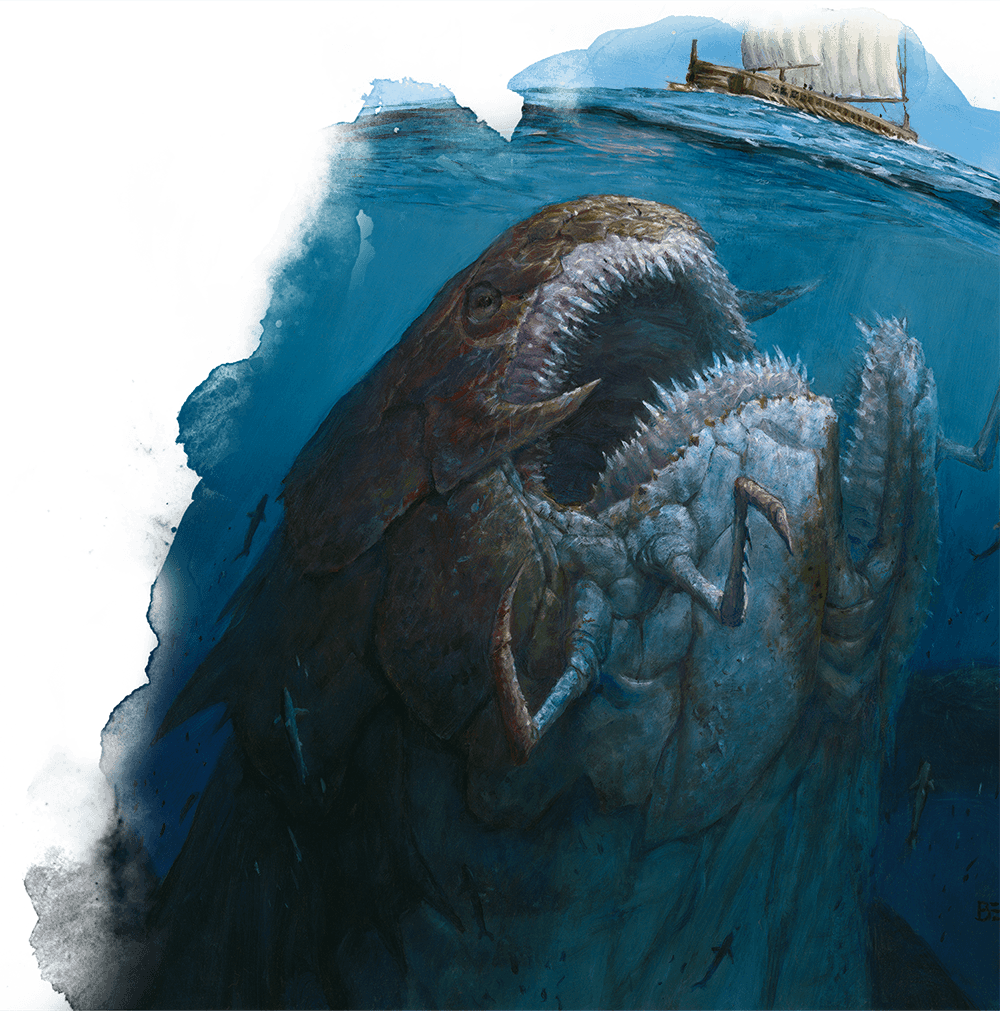
\includegraphics[width=0.5\pdfpagewidth]{03mechanics/img/41friendlyillhevi.png}};
    \end{tikzpicture}

    \newpage

    \begin{DndTable}[width=\linewidth, header=Cold]{cX}
        \textbf{d20} & \textbf{Effect} \\
        1     & Roll damage as normal. \\
        2-3   & The creature may only move half its movement speed on its next turn. \\
        4-6   & The creature has disadvantage on attack rolls until the end of its next turn. \\
        7-8   & The creature’s movement speed is 0 until the end of its next turn. \\
        9-11  & The creature gains vulnerability to bludgeoning damage for a minute. \\
        12-13 & The creature is paralyzed until the end of its next turn. \\
        14-16 & The creature is paralyzed until the end of its next turn.
        If the creature takes damage before the end of its next turn, roll on the minor injury chart. \\
        17-18 & The creature is paralyzed until the end of its next turn and rolls on the minor injury chart. \\
        19    & Roll on the major injury chart. \\
        20    & Roll on the major injury chart, and the creature is paralyzed for the next minute.
        The creature may attempt a Constitution saving throw at the end of each of its turns (DC 15) to end this effect.
        If it fails this saving throw three times it is frozen solid and becomes petrified, but frozen solid rather than turned to stone.
    \end{DndTable}

    \begin{DndTable}[width=\linewidth, header=Fire]{cX}
        \textbf{d20} & \textbf{Effect} \\
        1     & Roll damage as normal. \\
        2-3   & Attack rolls for attacks that deal fire damage have advantage against the creature until the end of its next turn. \\
        4-6   & You burn the creature's hands.
        The creature drops any objects it is holding. \\
        7-8   & The creature is on fire.
        While the creature is on fire it takes 2d4 fire damage at the start of each of its turns.
        The creature can end this condition by dropping prone and using 1 meter of movement to roll on the ground. \\
        9-11  &  \\
        12-13 & The creature is on fire.
        While the creature is on fire it takes 2d6 fire damage at the start of each of its turns.
        The creature can end this condition by dropping prone and using 1 meter of movement to roll on the ground. \\
        14-16 & The creature is charred.
        If the creature has resistance to fire, it loses that resistance.
        If the creature does not have resistance to fire, it gains vulnerability to fire.
        Both of these effects are considered a minor injury. \\
        17-18 & Roll on the minor injury chart.
        Additionally, the creature is on fire.
        While on fire it takes 2d6 fire damage at the start of each of its turns.
        The creature can end this condition by dropping prone and using 1 meter of movement to roll on the ground. \\
        19    & Roll on the major injury chart. \\
        20    & Roll on the major injury chart.
        Additionally, the creature is on fire.
        While the creature is on fire it takes 2d8 fire damage at the start of each of its turns.
        The creature can end this condition by dropping prone and using 1 meter of movement to roll on the ground.
    \end{DndTable}

    \begin{DndTable}[width=\linewidth, header=Force]{cX}
        % TODO. Check back here after done with spells. Dunno if we're keeping Force damage.
        \textbf{d20} & \textbf{Effect} \\
        1     & Roll damage as normal. \\
        2-3   & The creature has disadvantage on saving throws against spells until the end of its next turn. \\
        4-6   & The creature is pushed 3 meters away from you. \\
        7-8   & Spell attack rolls against the creature have advantage until the end of its next turn. \\
        9-11  & The creature is knocked prone. \\
        12-13 & The creature is spellbound until the end of its next turn.
        While spellbound it makes saving throws against spells with disadvantage and spell attack rolls against it have advantage. \\
        14-16 & The creature is spellbound for the next minute.
        While spellbound it makes saving throws against spells with disadvantage and spell attack rolls against it have advantage.
        At the end of each of the creature’s turns it can make an Intelligence saving throw (DC 12) to end this effect. \\
        17-18 & Roll on the minor injury chart.
        Additionally, the creature is spellbound for the next minute.
        While spellbound it makes saving throws against spells with disadvantage and spell attack rolls against it have advantage.
        At the end of each of the creature’s turns it can make an Intelligence saving throw (DC 15) to end this effect. \\
        19    & Roll on the major injury chart. \\
        20    & Roll on the major injury chart.
        Additionally, the creature is spellbound for the next minute.
        While spellbound it makes saving throws against spells with disadvantage and spell attack rolls against it have advantage.
        At the end of each of the creature’s turns it can make an Intelligence saving throw (DC 18) to end this effect.
    \end{DndTable}

    \begin{DndTable}[width=\linewidth, header=Lightning]{cX}
        \textbf{d20} & \textbf{Effect} \\
        1     & Roll damage as normal. \\
        2-3   & The creature cannot use reactions until the end of its next turn. \\
        4-6   & If the creature willingly moves before the start of your next turn, it takes 1d8 lightning damage. \\
        7-8   & You may choose one other creature within 4.5 m. of the victim.
        That creature must succeed on a Dexterity saving throw (DC 12) or take half as much damage. \\
        9-11  & The creature is paralyzed until the start of your next turn. \\
        12-13 & You may choose one other creature within 4.5 m. of the victim.
        That creature must succeed on a Dexterity saving throw (DC 15) or take half as much damage. \\
        14-16 & Roll on the minor injury chart.
        If the creature is wearing metal armor roll on the major injury chart instead. \\
        17-18 & The creature and all creatures within 4.5 m. of it cannot take reactions until the end of their next turn.
        Then roll on the minor injury chart. \\
        19    & Roll on the major injury chart. \\
        20    & All creatures within 4.5 m. of the victim must succeed on a Dexterity saving throw (DC 18) or take half as much damage.
        Then roll on the major injury chart.
    \end{DndTable}

    \begin{DndTable}[width=\linewidth, header=Necrotic]{cX}
        \textbf{d20} & \textbf{Effect} \\
        1     & Roll damage as normal. \\
        2-3   & The creature cannot regain hit points until the end of its next turn. \\
        4-6   & Choose an ability.
        The creature has disadvantage on ability checks made with the chosen ability for a minute. \\
        7-8   & The creature’s maximum hit points are reduced by an amount equal to the damage dealt.
        This lasts until the creature takes a short rest. \\
        9-11  & You heal yourself an amount equal to half of the damage dealt. \\
        12-13 & The creature’s maximum hit points are reduced by an amount equal to the damage dealt.
        This is considered a minor injury. \\
        14-16 & The creature cannot regain hit points for the next minute.
        It may make a Constitution saving throw (DC 15) at the end of each of its turns to end this effect. \\
        17-18 & The creature’s maximum hit points are reduced by an amount equal to the damage dealt.
        This is considered a major injury.
        Then roll on the minor injury chart. \\
        19    & Roll on the major injury chart. \\
        20    & The creature cannot regain hit points for the next minute.
        It may make a Constitution saving throw (DC 18) at the end of each of its turns to end this effect.
        Then roll on the major injury chart.
    \end{DndTable}

    \begin{DndTable}[width=\linewidth, header=Poison]{cX}
        \textbf{d20} & \textbf{Effect} \\
        1     & Roll damage as normal. \\
        2-3   & The creature has disadvantage on its next ability check, attack roll, or saving throw. \\
        4-6   & The creature stinks.
        It has disadvantage on all Charisma checks except Charisma (Intimidation) and Perception checks that rely on smell.
        This lasts until the creature bathes. \\
        7-8   & The creature has disadvantage on all ability checks, attack rolls, and saving throws until the end of its next turn. \\
        9-11  & Any creature in a radius of 2 meters around the target must roll a Constitution saving throw.
        On a failure, they take half the damage dealt. \\
        12-13 & The creature is poisoned for the next minute.
        The creature may attempt a Constitution saving throw at the end of each of its turns (DC 12) to end this effect. \\
        14-16 & The creature is poisoned for the next minute.
        The creature may attempt a Constitution saving throw at the end of each of its turns (DC 15) to end this effect. \\
        17-18 & Roll on the minor injury chart and the creature is poisoned for the next minute.
        The creature may attempt a Constitution saving throw at the end of each of its turns (DC 18) to end this effect. \\
        19    & Roll on the major injury chart. \\
        20    & Roll on the major injury chart, and the creature is poisoned for the next minute.
        The creature may attempt a saving throw at the end of each of its turns (DC 18) to end this effect.
    \end{DndTable}

    \begin{DndTable}[width=\linewidth, header=Psychic]{cX}
        \textbf{d20} & \textbf{Effect} \\
        1     & Roll damage as normal. \\
        2-3   & You control the creature’s movement on its next turn. \\
        4-6   & The creature cannot differentiate friend from foe until the end of its next turn. \\
        7-8   & Attacks against the creature are made with advantage until the start of your next turn. \\
        9-11  & You control the creature’s actions on its next turn. \\
        12-13 & The creature's mind is broken.
        If the creature has resistance to psychic damage, it loses that resistance.
        If the creature does not have resistance to psychic damage, it gains vulnerability to it.
        Both of these effects are considered a minor injury. \\
        14-16 & You control the creature during its next turn. \\
        17-18 & Roll on the Insanity chart with disadvantage. \\
        19    & Roll on the Insanity chart. \\
        20    & Roll on the Insanity chart with advantage.
    \end{DndTable}

    \begin{DndTable}[width=\linewidth, header=Radiant]{cX}
        \textbf{d20} & \textbf{Effect} \\
        1     & Roll damage as normal. \\
        2-3   & The has disadvantage on any Perception checks that rely on sight.
        This is considered a minor injury. \\
        4-6   & The creature's attack rolls are made with disadvantage. \\
        7-8   & The creature is blinded until the end of its next turn. \\
        9-11  & The creature is blinded for a minute.
        It can make a Constitution saving throw (DC 12) at the end of each of its turns to end this effect. \\
        12-13 & The creature glows for the next minute.
        While glowing it produces bright light up 2 meters and dim light up to 6 meters and all successful attacks against the creature deal an additional 1 radiant damage. \\
        14-16 & The creature is frightened of you for the next minute.
        It can make a Wisdom saving throw (DC 15) at the end of each of its turns to end this effect. \\
        17-18 & Roll on the minor injury chart.
        Additionally, the creature glows for the next minute.
        While glowing it produces bright light up 2 meters and dim light up to 6 meters and all successful attacks against the creature deal an additional 1d4 radiant damage. \\
        19    & Roll on the major injury chart. \\
        20    & Roll on the major injury chart.
        Additionally, the creature glows for the next minute.
        While glowing it produces bright light up 2 meters and dim light up to 6 meters and all successful attacks against the creature deal an additional 1d6 radiant damage.
    \end{DndTable}

    \pagebreak~
    \begin{tikzpicture}[remember picture,overlay]
        \node[anchor=north, yshift=0.10cm] at (current page.north) {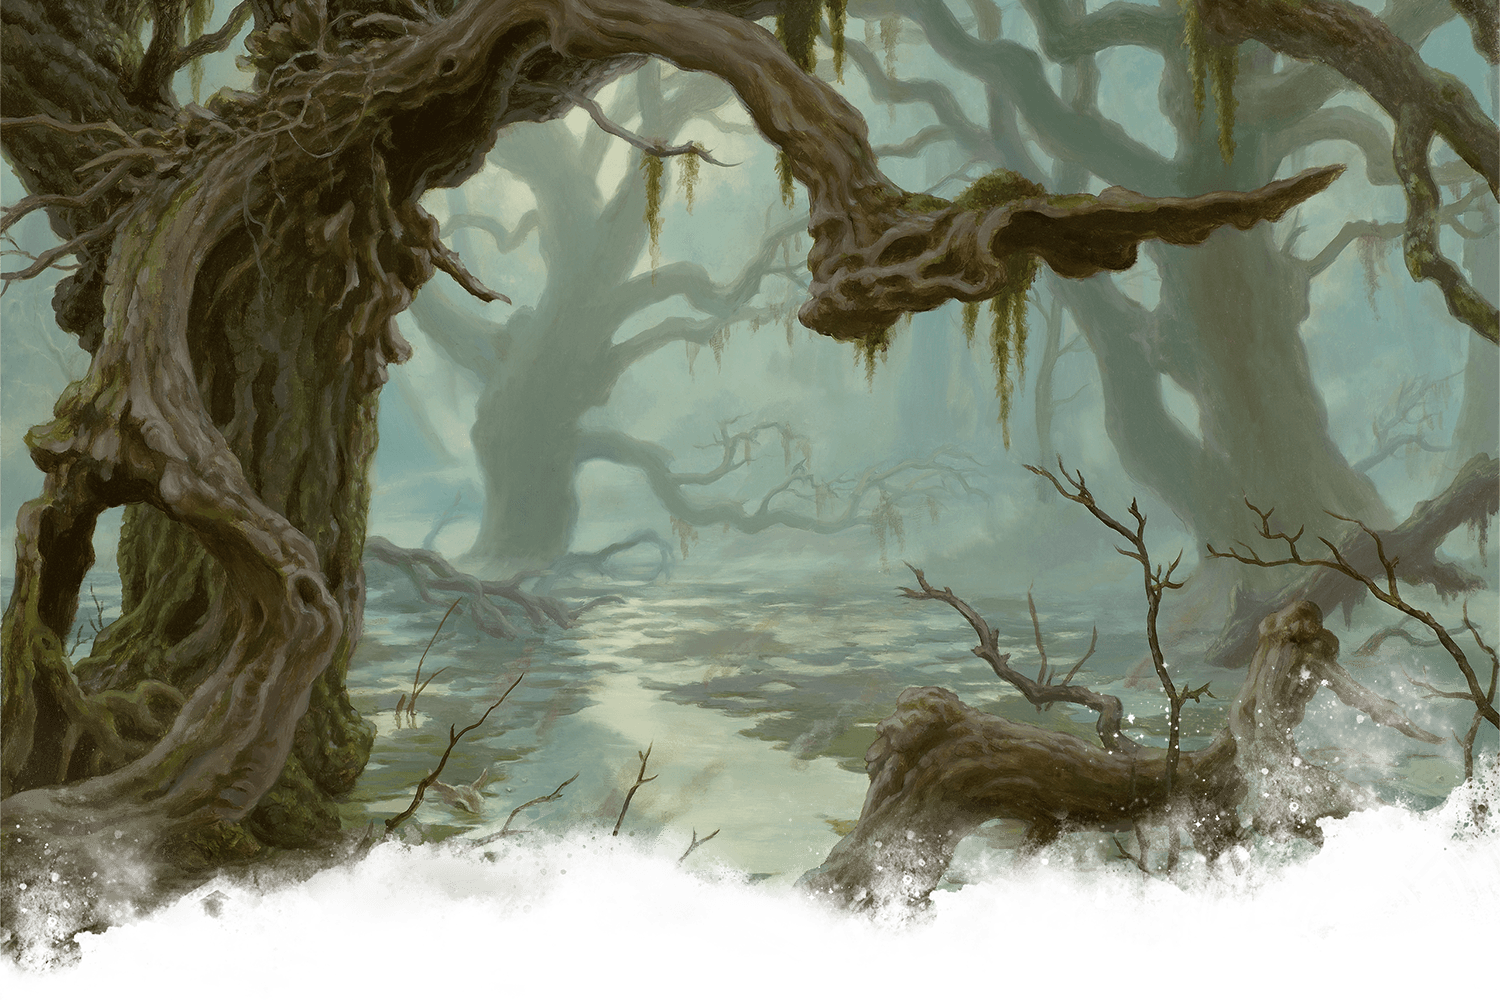
\includegraphics[width=\pdfpagewidth]{03mechanics/img/41arastas_domain.png}};
    \end{tikzpicture}

    \vspace{12.0cm}

    \begin{DndTable}[width=\linewidth, header=Thunder]{cX}
        \textbf{d20} & \textbf{Effect} \\
        1     & Roll damage as normal. \\
        2-3   & The creature has disadvantage on any Perception checks that rely on hearing.
        This is considered a minor injury. \\
        4-6   & The creature is deafened until the end of its next turn. \\
        7-8   & The creature is confused until the end of its next turn.
        While confused, the creature moves in a random direction determined by the DM. \\
        9-11  & The creature is deafened for one minute. \\
        12-13 & The creature is stunned until the start of its next turn and is deafened for one minute. \\
        14-16 & The creature is deafened permanently.
        This is considered a major injury. \\
        17-18 & The creature is stunned until the end of its next turn and is deafened for one minute.
        Then roll on the minor injury chart. \\
        19    & Roll on the major injury chart. \\
        20    & The creature is stunned until the end of its next round and is deafened for one minute.
        Then roll on the major injury chart.
    \end{DndTable}

% !TEX root = ../main.tex

\pagebreak~
\vspace{11.5cm}

\subsection*{Dementia} \label{ssec::dementia}
\DndDropCapLine{H}{arsh is the process that awaits the}
foolish or unlucky enough to lose their qualar.
Their sentience slips away slowly as they lose their mental capacities.
Perhaps the worst part is that inward awareness is one of the last attributes lost, forcing them to be fully conscious of the process.

The road towards dementia comes in seven stages, each roughly lasting a week.
At the moment when you lose your qualar, you enter the first stage of dementia.
After a week, you roll a DC 15 Intelligence saving throw.
On a fail, you enter the next stage of dementia.
On a success, you stay on your current stage and roll again at the start of the next week.
Dementia is unavoidable, and the DC increases by 1 after every successful roll.

\subsubsection{First Stage}
    No obvious signs of dementia, only minor short-memory loss occurs.
    The main symptoms are associated to the anxiety from the loss of the qualar.
    You start focusing more on your past, often drifting away into daydreams.

    You suffer the following effects:
    \subparagraph{Decreased Awareness} You roll for initiative and Dexterity saving throws with disadvantage.
    \subparagraph{Restlessness} Roll an DC 12 intelligence saving throw right after a short rest.
    On a success, you recover your hit points normally.
    On a failure, you only recover half of the hit dice rolled (rounded down).

\subsubsection{Second Stage}
    The self realization and awareness that something is wrong settles in.
    You refuse to accept that your mind is slipping away.
    The more effort you put on remembering the more deterioration your memory suffers.
    Confusion starts setting in.

    In addition to the effects of the first stage, you suffer the following effects:
    \subparagraph{Lack of Recollection} Any ability check made to remember or recollect a memory is done with disadvantage.
    All Intelligence (History) checks are made with disadvantage.
    \subparagraph{Mood Swings} All Charisma ability checks and saving throws are made with disadvantage.

\subsubsection{Third Stage}
    You experience increased forgetfulness and might find concentrating difficult.
    You are presented with some of the last coherent memories before confusion fully rolls in.
    Some singular memories become more disturbed, isolated, broken, and distant.
    These are the last embers of awareness.

    In addition to the effects of the last stages, you suffer the following effects:
    \subparagraph{Decreased Concentration} All Constitution saving throws made to maintain concentration are made with disadvantage.
    \subparagraph{Vagrant Mind} Intelligence and Wisdom ability checks and saving throws are rolled with disadvantage.

\subsubsection{Fourth Stage}
    Grey mists form and fade away in your memory.
    The ability to recall singular memories gives way to confusion and horror.
    You struggle with daily tasks, presenting clear cognitive problems.

    In addition to the effects of the last stages, you suffer the following effects:
    \subparagraph{Motor Difficulties} Strength and Dexterity ability checks and saving throws are rolled with disadvantage.
    Attack rolls are made with disadvantage.
    \subparagraph{Drifting Conscience} In combat, roll a DC 8 Intelligence saving throw at the start of every turn.
    On a failure, you forget where you are, and cannot take any actions during the turn.

\subsubsection{Fifth Stage}
    You have major memory deficiencies.
    The few lapses of consciousness you get are filled with dread, as you realize your mind has mostly left you.
    The repetition and rupture gives way to calmer moments, as the unfamiliar becomes familiar.

    In addition to the effects of the last stages, you suffer the following effects:
    \subparagraph{Loss of Fortitude} All rolls are made with disadvantage.
    \subparagraph{Complete Unawareness} All Intelligence (Investigation), Wisdom (Insight), and Wisdom (Perception) automatically fail.
    Your passive investigation, insight, and perception become 0.

\subsubsection{Sixth Stage}
    Your mental state is beyond description.
    You struggle to remember your early life, even forgetting the names of your family and fellows.
    Your capacity of speech is severely impaired, and you suffer sudden and radical personality and emotional changes.

    In addition to the effects of the last stages, you suffer the following effects:
    \subparagraph{Declining Speech} You automatically fail all Charisma ability checks and saving throws, and have a very hard time communicating verbally.
    \subparagraph{Hope Lost} As your conscious mind fights your natural tendencies, you automatically fail death saving throws.

\subsubsection{Final Stage}
    Everywhere, an empty bliss.

    You make what will most likely be your last die roll.
    Nothing can give you advantage or disadvantage on this roll.
    Roll a d20 on the post-dementia table.
    You suffer the effect rolled.

    \begin{DndTable}[width=\linewidth, header=Post-dementia Effects]{lX}
        \textbf{Roll} & \textbf{Effect} \\
        1 & Your last emotion is rage.
        You become mindless and violent, attacking your companions without reason. \\
        2-5 & Your last emotion is apathy.
        You mindlessly stare to the east until you die of natural causes. \\
        6-18 & Even after brain death, you seek survival.
        You wander off, attacking any who try to stop you.
        You become a lost one. \\
        19 & With memories gone, your mind is fully pulled by its tidal impulses.
        You lose control of your character, who becomes a servant of The Sorrow. \\
        20 & Recovery from dementia is very rare, but not impossible.
        You recover from all effects associated to dementia, and gain the \textbf{Demented Insight} feat.
    \end{DndTable}

    The only conventional way to remove dementia is to obtain a qualar again.
    When this happens, you quickly recover your sentience.
    Each morning, you reduce your stage of dementia by one, and don't need to roll the Intelligence saving throw associated to the status.

    \subsubsection{Demented Insight} \label{feat::dementedinsight}
    A true master of the mind, you are able to retain your sentience without a qualar.
    You are immune to the effects of dementia.


% \pagebreak~
% \begin{tikzpicture}[remember picture,overlay]
%     \node[anchor=north, yshift=0.10cm] at (current page.north) {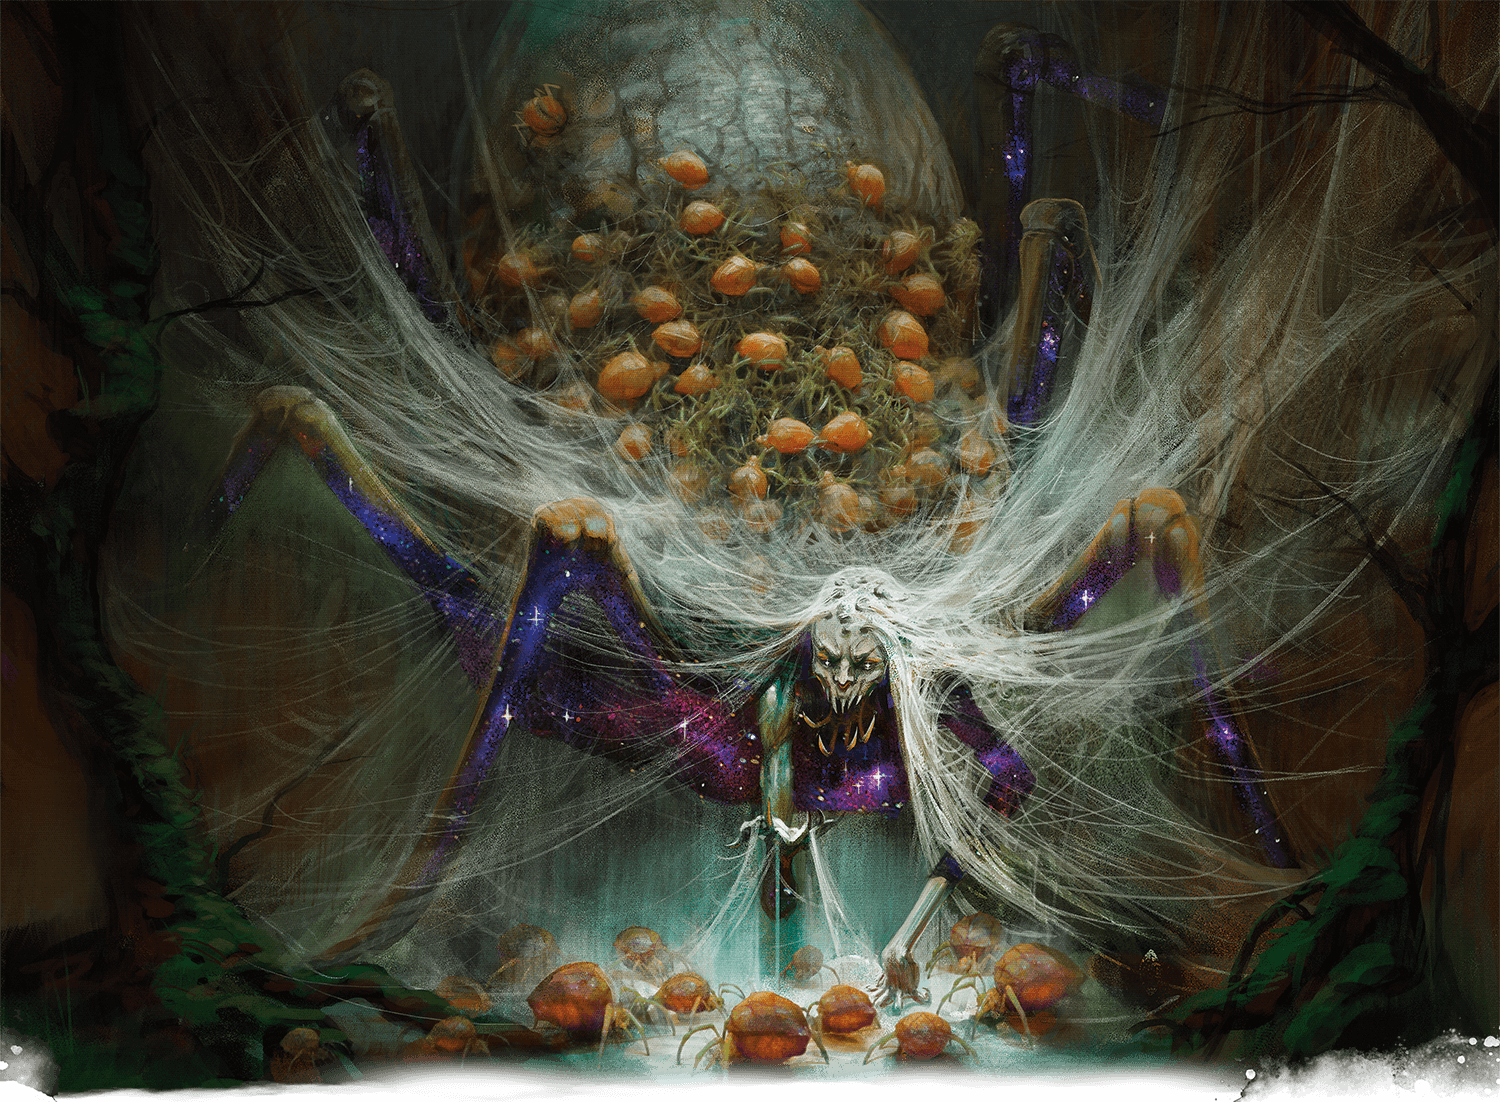
\includegraphics[width=\pdfpagewidth]{03mechanics/img/40arastaoftheendlessweb.png}};
% \end{tikzpicture}
%
% \vspace{14.0cm}

\subsection*{Flaws} \label{ssec::flaws}
    As you travel through treacherous lands and fight dangerous creatures, it is natural to acquire permanent wounds or fears.
    These new flaws don't need to be entirely bad --- they reflect a changing point in your life, and can be beneficial in their own way.

    When you suffer a major injury, fear, or insanity, you can choose to accept this effect as a flaw.
    When you do so, it becomes permanent.
    For example, a crippled arm might need to be severed off, or your character might get used to their insanity and learn to live with it instead of treating it.

    While this effect may prove as a permanent hindrance to you, you are rewarded with FP for taking it.
    This extra FP does not count towards your level.
    The number of FP awarded by effects is specified in the effect's description.

% \pagebreak~
% \vspace{11.5cm}

\subsection*{Injuries \& Insanity} \label{ssec::injuriesandinsanity}
    Critical hits or especially severe events can cause injuries or insanity.
    When a creature suffers a minor injury it can be healed by someone competent with a healer's kit over the course of a long rest.
    Major injuries and Insanities require assistance from a dedicated healer, or someone with the relevant feat (see page \pageref{feat::physician} and \pageref{feat::therapist}).

    Alternatively, you can decide to keep an injury or insanity as a new Flaw (see page \pageref{ssec::flaws}) during a short rest after it is applied.
    Minor injuries and insanities award you 2 FP, while major injuries award you 3 FP.
    Acquiring a flaw from a major injury related to a minor injury you already have (such as Crippled Leg and Injured Leg) only awards 1 FP --- one more than what you already had gained.
    % The text of certain injuries will specify other ways this injuries might resolve.

    % \pagebreak

    \begin{table*}[t]
        \begin{DndTable}[width=\linewidth, header=Minor and Major Injuries]{cXX}
            \textbf{d20} & \textbf{Minor Injury} & \textbf{Major Injury} \\
            1-3 &
            \textbf{Injured leg}.
            Your movement speed is reduced by 2 meters. &
            \textbf{Crippled leg}.
            Your movement speed is reduced by 2 meters, and you have disadvantage on Dexterity saving throws. \\
            4-8 &
            \textbf{Injured arm}.
            One of your arms (randomly determined) cannot be used to hold a shield, and you have disadvantage on any rolls involving the use of that arm. &
            \textbf{Crippled arm}.
            One of your arms (randomly determined) cannot be used to hold an item, and any ability check or attack roll requiring that arm automatically fails. \\
            9-11 &
            \textbf{Multiple injuries}.
            Your maximum hit points are reduced by an amount equal to half of the damage dealt by the attack. &
            \textbf{Severely wounded}.
            Your maximum hit points are reduced by an amount equal to the damage dealt by the attack. \\
            12-16 &
            \textbf{Badly beaten}.
            You have disadvantage on Constitution saving throws. &
            \textbf{Edge of death}.
            You have disadvantage on Constitution and death saving throws. \\
            17-19 &
            \textbf{Ringing blow}.
            You are stunned until the end of your next turn, and you are deafened. &
            \textbf{Blinding blow}.
            You are blinded. \\
            20    &
            \textbf{Blow to the head}
            You are unconscious for 2d12 hours. &
            \textbf{Decapitated}.
            You are dead.
        \end{DndTable}
    \end{table*}

    % \thispagestyle{empty} % Remove footer so that it doesn't clash with the image.
    % \begin{tikzpicture}[remember picture,overlay]
    %     \node[anchor=south west, xshift=-0.10cm, yshift=-0.10cm] at (current page.south west) {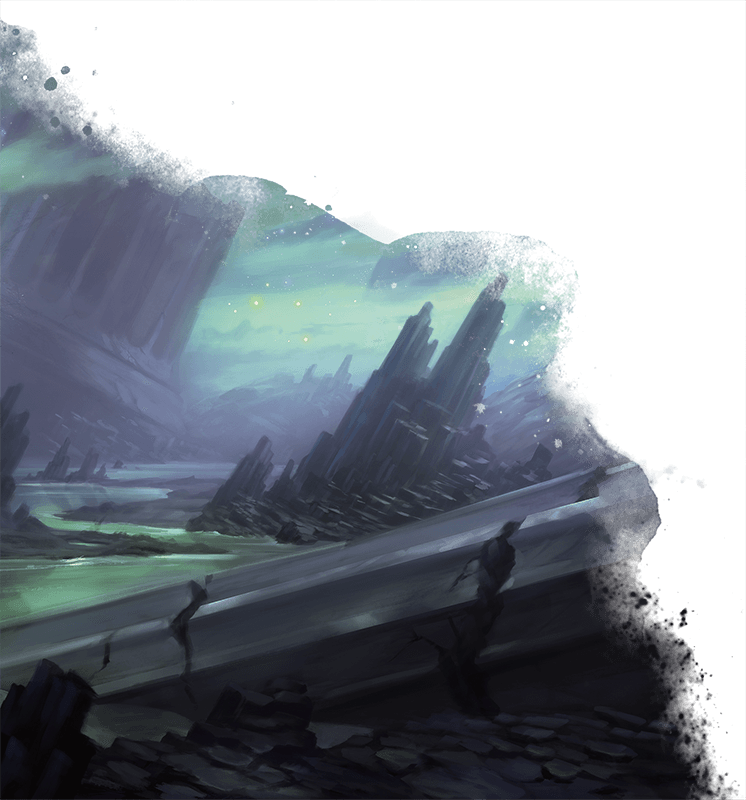
\includegraphics[width=0.5\pdfpagewidth]{03mechanics/img/40outerlands.png}};
    % \end{tikzpicture}

\subsection*{Only One Chance} \label{ssec::onlyonechance}
    As a rule, you only have one chance to succeed in any action.
    Once you have rolled the dice, you many not roll again to achieve the same goal.
    You need to try something different or wait until the circumstances have changed in a substantial way.
    Or, you know, let another PC try.

    This rule does not apply to combat, where you can attack the same enemy until it becomes a bloody pulp.

\subsection*{Opportunity Attacks} \label{rule::opportunityattacks}
    In a fight, everyone is constantly watching for enemies to drop their guard.
    While heedless movement is easily punished, any lack of concentration or unplanned action can have devastating consequences.
    Various actions provoke opportunity attacks from a creature:
    \begin{itemize}
        \item Moving out of the creature's reach.
        This doesn't apply when someone or something moves you without using your movement, action, or reaction.

        % \newpage

        \item Picking up an item from the floor while in the creature's reach.
        \item Unsheathing a weapon while in the creature's reach.
        \item Donning or doffing a shield while in the creature's reach.
        \item Using the Attack action with a ranged weapon or spell attack in a creature's reach.
    \end{itemize}
    You can avoid opportunity attacks during your turn by taking the Disengage action.

\subsection*{Short and Long Rests} \label{ssec::shortandlongrests}
    The gritty campaigns in Yuadrem benefit from longer rest times.
    Short rests last for 8 hours, and long rests for 3 days --- half a week in the Fagalian calendar.
    This puts the brakes on the campaign, requiring the players to carefully judge the benefits and drawbacks of combat.
    % Characters can't afford to engage in too many battles in a row, and all adventuring requires careful planning.

    Complementing this optional rule is the fact that all spell slots are recovered during short rests, and a short rest removes one level of exhaustion.
    Additionally, all the systems in this book are designed with this optional rule in mind, so some things need to be re-balanced if a group is to play without this rule.

    \begin{table*}[h]
        \begin{DndTable}[width=\linewidth, header=Insanity]{cX}
            \textbf{d20} & \textbf{Insanity} \\
            1  & \textbf{Synesthesia}.
            You can hear colors, smell sounds, or taste textures. Regardless of the specific manifestation, you have disadvantage on all Perception and Investigation skill checks. \\
            2  & \textbf{Kleptomania}.
            Once per day when you are in a personal residence or marketplace, the DM can call on you to succeed on a Wisdom saving throw (DC 12) or attempt to steal an item of insignificant practical and monetary value. \\
            3  & \textbf{Paranoia}.
            Once per day following an interaction with another creature (including other PCs) the DM can call on you to succeed on a Wisdom saving throw (DC 12) or you suspect that creature is secretly plotting against you. \\
            4  & \textbf{Obsession}.
            Choose a person or personal interest you are obsessed with. Once per day, when you are presented with an opportunity to interact with or learn more about the subject of your obsession the DM can call on you to succeed on a Wisdom saving throw (DC 14) or ignore everything else to obsess over the object of your fascination. \\
            5  & \textbf{Addiction}.
            Choose a behavior or substance you have used. Once per day, when you are presented with an opportunity to do the behavior or use the substance the DM can call on you to succeed on a Wisdom saving throw (DC 14) or ignore everything else to indulge in your vice. \\
            6  & \textbf{Odd Thinking}.
            Once per day when you hear a rational explanation for an event or occurrence, your DM may call on you to succeed on a Wisdom saving throw (DC 12) or you reject the rational explanation for a conspiratorial or fantastical explanation. \\
            7  & \textbf{Narcissism}.
            When you take an action or series of action that doesn't directly benefit you, you must pass a Wisdom saving throw (DC 11) or you can’t take that action / series of actions.
            If any self-sacrifice on your part would be required the DC of the saving throw is increased to 16. \\
            8  & \textbf{Delusional}.
            When you gain this insanity the DM will tell you a belief that you have. No matter what evidence is presented to the contrary so long as you have this insanity you cannot be persuaded that this belief is not true. \\
            9  & \textbf{Pica}.
            Once per day the DM can call on you to pass a Wisdom saving throw (DC 14) or immediately eat one non-food object (such as dirt, napkins, or a small piece of jewelry) of the DM’s choice. \\
            10 & \textbf{Retrograde amnesia}.
            You forget everything about your personal life prior to the moment you received this insanity. \\
            11 & \textbf{Overwhelmed}.
            If you do not have immunity or resistance to psychic damage, you gain vulnerability to psychic damage.
            If you have resistance to psychic damage, you lose it.
            If you have immunity to psychic damage, you lose it but gain resistance to psychic damage. \\
            12 & \textbf{Anterograde amnesia}.
            Whenever you try to recall a fact you learned since you received this insanity, make a Intelligence saving throw (DC 12).
            If you fail you cannot recall the fact. \\
            13 & \textbf{Dependence}.
            You must pass a Wisdom saving throw (DC 14) to take an action that one or more of your allies disapprove of. \\
            14 & \textbf{Anxious}.
            You have disadvantage on saving throws against being frightened.
            Additionally, once per day the DM can call on you to succeed a Wisdom saving throw (DC 14) or be frightened by a creature of the DM’s choosing for the next minute. \\
            15 & \textbf{Mute}.
            Whenever you wish to speak allowed (including casting a spell that has verbal components) you must succeed on a Wisdom saving throw (DC 13) to do so. \\
            16 & \textbf{Narcolepsy}.
            You have disadvantage on saving throws against sleeping or unconsciousness.
            Once per day the DM may call on you to succeed on a Constitution saving throw (DC 12) or fall unconscious for one minute or until you take damage or another creature spends their action trying to rouse you. \\
            17 & \textbf{Insomnia}.
            You cannot take long rests and your short rests take 8 hours to complete. \\
            18 & \textbf{Homicidal}.
            After each long rest you must pass a Wisdom saving throw (DC 14) or be overcome with the urge to end the life of a humanoid creature and you cannot benefit from another long rest until you do so. \\
            19 & \textbf{Suicidal}.
            After each long rest you must pass a Wisdom saving throw (DC 12) or make an attempt to end your own life. \\
            20 & \textbf{Catatonia}.
            You are unconscious for 10d10 years.
        \end{DndTable}
    \end{table*}

\subsection*{Stress} \label{ssec::stress}
    Adventuring is dangerous, and no matter the amount of heroic deeds in your past you are bound to accumulate stress over time.
    As a mechanic, stress adds long-term consequences to traumatic experiences and tense situations.

    Whenever you drop to 0 hit points, add a point to your stress meter.
    % Some specific attacks directly produce stress on a creature.
    When you reach 4 stress points, you roll on the Afflictions table and acquire the specified affliction, reducing your stress meter back to 2.
    % Afflictions are detrimental conditions that have short or long-term consequences for you.

    Taking a long rest or engaging in downtime activities reduces your stress meter by 1.
    Additionally, some feats like Soothing Presence (see page \pageref{feat::soothingpresence}) and Reliever (see page \pageref{feat::reliever}) add the capacity to reduce stress in different scenarios.

    % \newpage~\newpage~\newpage

    \begin{table*}[t]
    \begin{DndTable}[width=\linewidth, header=Affliction]{cX}
        \textbf{d20} & \textbf{Affliction} \\
        1     & \textbf{Insanity}.
        Your mind collapses and you fall into insanity.
        Roll on the Insanity table (see page \pageref{ssec::injuriesandinsanity}) and acquire the rolled insanity. \\
        2-5   & \textbf{Phobia}.
        Powerless at the face of death, you can only watch as your foe strikes its final blow against you.
        You add to your flaws the phobia of the type of creature who put you unconscious.
        Any time you encounter this type of creature, roll a DC 16 Wisdom saving throw at the beginning of each of your turns.
        On a failure, you become frightened of the creature.
        This flaw is permanent, and awards you 1 FP. \\
        6-7   & \textbf{Fearful}.
        % Scared of death, you become fearful and meek.
        Whenever you take damage, roll a DC 12 Wisdom saving throw.
        On a failure, you become frightened of the attacking creature.
        You can repeat this saving throw at the end of each turn.
        This effect lasts until you finish a short rest. \\
        8-9   & \textbf{Paranoid}.
        Whenever you are targeted by a friendly creature for any effect, roll a DC 12 Wisdom saving throw.
        On a failure, you refuse what your ally is offering, be it healing, aid, etc.
        If you ally spent any resource or action on this effect, they are spent anyway.
        This effect lasts until you finish a short rest. \\
        10-11 & \textbf{Selfish}.
        You cannot heal or aid an ally in any way.
        This effect lasts until you finish a short rest. \\
        12-13 & \textbf{Masochistic}.
        Your AC is reduced by 2, and you cannot take the Dodge or Disengage actions.
        This effect lasts until you finish a short rest. \\
        14-15 & \textbf{Abusive}.
        You cannot heal or aid an ally in any way, and you refuse to receive any healing or aid from any creature.
        This effect lasts until you finish a short rest. \\
        16-17 & \textbf{Hopeless}.
        Attacks against you are made with advantage, and you roll saving throws with disadvantage.
        This effect lasts until you finish a short rest. \\
        18-19 & \textbf{Irrational}.
        At the beginning of each of your turns, roll a DC 15 Wisdom saving throw.
        On a failure, you cannot take any action during your turn.
        This effect lasts until you finish a short rest. \\
        20    & \textbf{Virtuous}.
        Stalwart against adversity, your time at death's door only enhances your resolution.
        Your stress meter is reduced to 0, and any ally that can see or hear you has their stress meter reduced by 1.
        Additionally, you have advantage on attack rolls and saving throws for one hour.
    \end{DndTable}
    \end{table*}

    % \thispagestyle{empty}
    % \begin{tikzpicture}[remember picture,overlay]
    %     \node[anchor=south, yshift=-0.10cm] at (current page.south) {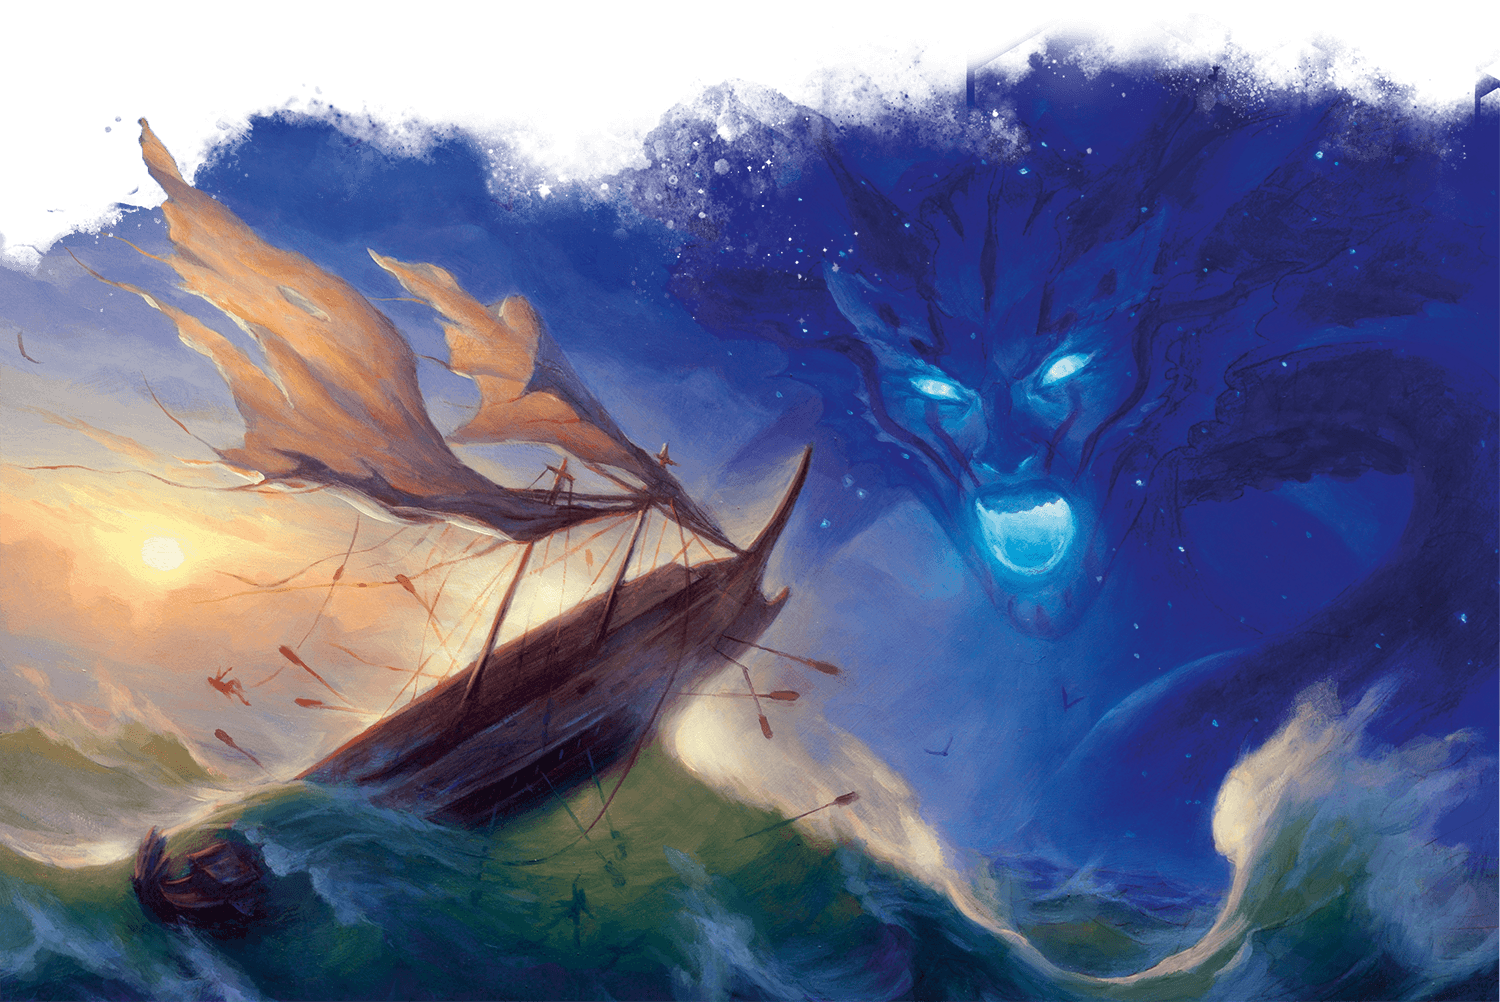
\includegraphics[width=\pdfpagewidth]{03mechanics/img/40thassaangry.png}};
    % \end{tikzpicture}
